\section{Operational Amplifiers}\label{sec:Op-Amps}
\begin{definition}[Op-Amp]\label{def:Op-Amp}
  An \emph{op-amp}, (\emph{operational amplifier}), is a active circuit element that is a 2-port network element.
  An circuit symbol for an op-amp is shown in \Cref{fig:Op-Amp}.
\end{definition}

\begin{figure}[h!tbp]
  \centering
  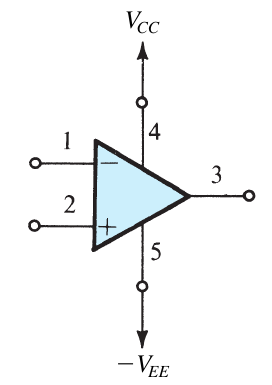
\includegraphics[scale=0.85]{./Op-Amp.png}
  \caption{Complete Circuit Symbol for an Op-Amp \parencite[p.~60]{sedraTextbook7}}
  \label{fig:Op-Amp}
\end{figure}


%%% Local Variables:
%%% mode: latex
%%% TeX-master: "../ECE_311-Engineering_Electronics-Reference_Sheet"
%%% End:
